%Chapter 2

\chapter{Literature Review} % Main chapter title

\label{literature} % For referencing the chapter elsewhere, use \ref{Chapter1} 

\lhead{Chapter 2. \emph{Literature Review}} % This is for the header on each page - perhaps a shortened title

%----------------------------------------------------------------------------------------
This chapter gives a background and a literature of the previous work, ~\ref{sec:sim} shows different existing similarity techniques, while section ~\ref{sec:clustering}  shows the exiting clustering algorithms and the advantages and disadvantages of each one, finally section ~\ref{sec:reco} discuss the existing recommending systems.
\section{Semantic Similarity}\label{sec:sim}, 
The problem of formalizing and quantifying the intuitive notion of similarity has a long history in philosophy, psychology, and artificial intelligence, and many different perspectives have been suggested. Recent research on the topic in computational linguistics has emphasized the perspective of semantic relatedness of two lexemes in a lexical resource, or its inverse, semantic distance. It’s important to note that semantic relatedness is a more general concept than similarity; similar entities are usually assumed to be related by virtue of their likeness (bank - trust company), but dissimilar entities may also be semantically related by lexical relationships such as metonymy (car - wheel) and antonymy (hot - cold), or just by any kind of functional relationship or frequent association (pencil - paper, penguin - Antarctica).\\

Measures of text similarity have been used for a long time in applications in natural language processing and related areas. Text similarity has been also used for relevance feedback and text classification (Rocchio, 1971), word sense disambiguation (Lesk, 1986), and more recently for extractive summarization (Salton et al., 1997b), and methods for automatic evaluation of machine translation (Papineni et al., 2002) or text summarization (Lin and Hovy, 2003). \\
The typical approach to finding the similarity between two text segments is to use a simple lexical matching method, and produce a similarity score based on the number of lexical units that occur in both input segments. \\
Improvements to this simple method have considered stemming, stop-word removal, part-of-speech tagging, longest subsequence matching, as well as various weighting and normalization factors (Salton et al., 1997a).\\
While successful to a certain degree, these lexical matching similarity methods fail to identify the semantic similarity of texts. For instance, there is an obvious similarity between the text segments I own a dog and I have an animal, but most of the current text similarity metrics will fail in identifying any kind of connection between these texts. \\

The only exception to this trend is perhaps the latent semantic analysis (LSA) method (Landauer et al., 1998), which represents an improvement over earlier attempts to use measures of semantic similarity for information retrieval (Voorhees, 1993), (Xu and Croft, 1996). LSA aims to find similar terms in large text collections, and measure similarity between texts by including these additional related words. \\
However, to date LSA has not been used on a large scale, due to the complexity and computational cost associated with the algorithm, and perhaps also due to the “black-box” effect that does not allow for any deep insights into why some terms are selected as similar during the singular value decomposition process.\\

On the other hand, another group of approaches that gaines wide approval is the Knowledge-based group. Knowledge-based can be explained as a measure of semantic similarity between words, and an indication of the word specificity.\\

%----------------------------------------------------------------------------------------
\section{Clustering}\label{sec:clustering}
Clustering is the unsupervised classification of patterns (observations, data items, or feature vectors) into groups \textit{clusters}, such that items within a cluster are very similar and items in different clusters are very different.

\subsection{Document clustering}
Document clustering has been investigated for use in a number of different areas of text
mining and information retrieval. Initially, document clustering was investigated for improving
the precision or recall in information retrieval systems and as an efficient way of
finding the nearest neighbors of a document. More recently, clustering has been
proposed for use in browsing a collection of documents or in organizing the results
returned by a search engine in response to a user’s query. Document clustering has
also been used to automatically generate hierarchical clusters of documents. The
automatic generation of a taxonomy of Web documents like that provided by Yahoo!

\citep{clustering_15} For most of clustering algorithms documents are represented using the vector-space model. In
this model, each document, $d$, is considered to be a vector, $d$, in the term-space (set of document
“words”). In its simplest form, each document is represented by the (TF) vector,
$d_{tf} = (tf_1, tf_2,..., tf_n)$, where $tf_i$ is the frequency of the $i^{th}$ term in the document. (Normally very common words are
stripped out completely and different forms of a word are reduced to one canonical form.) In
addition, other variation of this model that weights each term based on its inverse document is used.

In this work we used clustering to group similar documents together and to determine the user neighborhood which affects the scalability of large scale recommender system. The clustering uses one of the different similarity metrics introduced in chapter ~\ref{sim} which reflects the semantic relatedness between articles.
\subsection{Clustering algorithms types}
Different approaches to clustering data can be described with the help of the hierarchy shown in Figure ~\ref{fig:clustering_approaches}

\begin{figure}[htbp]
	\centering
		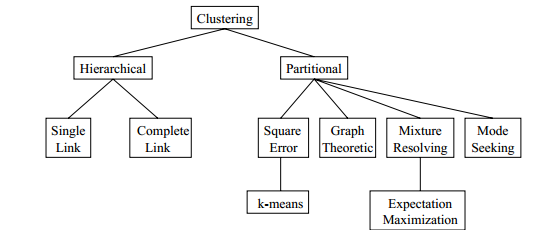
\includegraphics{./Figures/clustering.png}
		\rule{35em}{0.5pt}
	\caption[Clustering techniques]{Clustering techniques}
	\label{fig:clustering_approaches}
\end{figure}

\subsubsection{Partitional}
Given a database of objects, a partitional clustering algorithm constructs
partitions of the data, where each cluster optimizes a clustering criterion, such as the minimization of the sum of squared distance from the mean within each cluster.
One of the issues with such algorithms is their high complexity, as some of them exhaustively enumerate
all possible groupings and try to find the global optimum. Even for a small number of objects,
the number of partitions is huge. That’s why, common solutions start with an initial, usually
random, partition and proceed with its refinement. A better practice would be to run the partitional algorithm for different sets of initial points (considered as representatives) and investigate whether all solutions lead to the same final partition.
Partitional Clustering algorithms try to locally improve a certain criterion. First, they compute the
values of the similarity or distance, they order the results, and pick the one that optimizes the criterion.Hence, the majority of them could be considered as greedy-like algorithms.


A major drawback of both of these schemes is that they fail for data in which points in a given cluster are closer
to the center of another cluster than to the center of their own cluster \citep{clustering_14}, as shown in figure ~\ref{fig:kmeans_fail}

\begin{figure}[htbp]
	\centering
		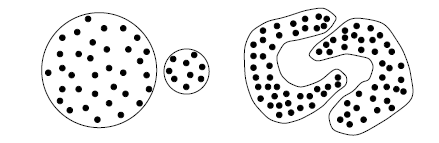
\includegraphics{./Figures/clustering_2.png}
		\rule{35em}{0.5pt}
	\caption[Data sets on which centroid and medoid approaches fail.]{Data sets on which centroid and medoid approaches fail.}
	\label{fig:kmeans_fail}
\end{figure}


\subsubsection{Hierarchical}
Hierarchical algorithms create a hierarchical decomposition of the objects. They are either
agglomerative (bottom-up) or divisive (top-down):
\paragraph{Agglomerative algorithms}
Agglomerative algorithms start with each object being a separate cluster itself, and successively
merge groups according to a distance measure. The clustering may stop when all objects are in
a single group or at any other point the user wants.
These methods generally follow a greedy-like bottom-up merging.
A major limitation of existing agglomerative hierarchical schemes such as the Group Averaging Method,
ROCK, and CURE is that the merging decisions are based upon static modeling of the clusters to
be merged. The selection mechanism of CURE (and of the single link method) (as illustrated in figure ~\ref{fig:hir_fail})will prefer merging clusters (a) and (b) over merging clusters (c) and (d), since the minimum distances between the representative points of (a) and (b) will be smaller than those for clusters (c) and
(d). But clusters (c) and (d) are better candidates for merging because the minimum distances between the boundary
points of (c) and (d) are of the same order as the average of the minimum distances of any points within these clusters
to other points. Hence, merging (c) and (d) will lead to a more homogeneous and natural cluster than merging (a) and
(b).
\begin{figure}[htbp]
	\centering
		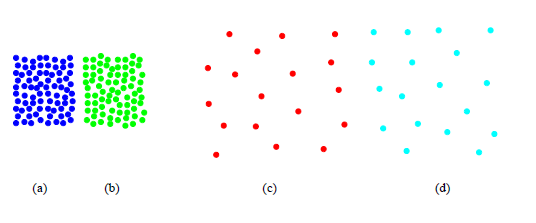
\includegraphics{./Figures/clustering_3.png}
		\rule{35em}{0.5pt}
	\caption[Example of clusters for merging choices.]{Example of clusters for merging choices.}
	\label{fig:hir_fail}
\end{figure}

\paragraph{Divisive algorithms} Divisive algorithms follow the opposite strategy. They start with one group of all objects and
successively split groups into smaller ones, until each object falls in one cluster, or as desired.
Divisive approaches divide the data objects in disjoint groups at every step, and follow the same
pattern until all objects fall into a separate cluster. This is similar to the approach followed by
divide-and-conquer algorithms.
Partitional and hierarchical methods can be integrated. This would mean that a result given by a hierarchical
method can be improved via a partitional step, which refines the result via iterative relocation
of points.



Apart from the two main categories of  partitional and hierarchical clustering algorithms, many other methods
have emerged in cluster analysis, and are mainly focused on specific problems or specific data sets
available. These methods include:

\subsubsection{Grid-Based Clustering} The main focus of these algorithms is spatial data, i.e., data that model the geometric
structure of objects in space, their relationships, properties and operations. The objective of
these algorithms is to quantize the data set into a number of cells and then work with objects belonging
to these cells. They do not relocate points but rather build several hierarchical levels of groups of
objects. In this sense, they are closer to hierarchical algorithms but the merging of grids, and consequently
clusters, does not depend on a distance measure but it is decided by a predefined parameter.

\subsubsection{Model-Based Clustering} These algorithms find good approximations of model parameters that best fit
the data. They can be either partitional or hierarchical, depending on the structure or model they
hypothesize about the data set and the way they refine this model to identify partitionings. They
are closer to density-based algorithms, in that they grow particular clusters so that the preconceived
model is improved. However, they sometimes start with a fixed number of clusters and they do not
use the same concept of density.
\subsubsection{Categorical Data Clustering} These algorithms are specifically developed for data where Euclidean, or
other numerical-oriented, distance measures cannot be applied. In the literature, we find approaches
close to both partitional and hierarchical methods.

\subsubsection{Density-Based Clustering} 
The problem of detecting clusters of points in data is challenging when the clusters are of 
different size, density and shape. Many of these issues become even more significant when 
the data is of very high dimensionality and when it includes noise and outliers. 

Density-Based Clustering algorithms group objects according to specific density objective functions.
Density is usually defined as the number of objects in a particular neighborhood of a data objects.
In these approaches a given cluster continues growing as long as the number of objects in the
neighborhood exceeds some parameter. This is considered to be different from the idea in partitional
algorithms that use iterative relocation of points given a certain number of clusters.


\paragraph{(DBSCAN) Density-Based Spatial Clustering of Applications with Noise} DBSCAN is most widely used density based algorithm. It uses the concept of  density reachability and density connectivity\citep{literature_1}. where
\begin{itemize}
\item{Density Reachability} A point $p$ is said to be density reachable from a point $q$ if point $p$ is within $\epsilon$ distance from point $q$ and $q$ has sufficient number of points in its neighbors which are within distance $\epsilon$ .

\item{Density Connectivity} A point $p$ and $q$ are said to be density connected if there exist a point $r$ which has sufficient number of points in its neighbors and both the points $p$ and $q$ are within the $\epsilon$ distance. This is chaining process. So, if $q$ is neighbor of $r$, $r$ is neighbor of $s$, $s$ is neighbor of $t$ which in turn is neighbor of $p$ implies that $q$ is neighbor of $p$.
\end{itemize}

\paragraph{The algorithm:}

\citep{literature_2}  The key idea of the DBSCAN algorithm is that, for each point of a cluster, the neighbourhood 
of a given radius has to contain at least a minimum number of points, that is, the density in 
the neighbourhood has to exceed some predefined threshold. This algorithm needs three 
input parameters:
\begin{itemize}  
\item{$k$, the neighbour list size} 
\item{$Eps$, the radius that delimitate the neighbourhood area of a point ($Epsneighbourhood$)}
\item{MinPts, the minimum number of points that must exist in the Eps-neighbourhood.}
\end{itemize} 

\subsubsection{Dynamic-model clustering algorithms}
The clustering process is based on the classification of the points in the dataset as  core 
points,  border points and  noise points, and on the use of density relations between points 
(directly density-reachable,  density-reachable,  density-connected) to form the 
clusters. 

The previous algorithms use a static model which refers to using user-defined parameters for defining density thresholds without referring to the characteristics of the underlying data. These algorithms can breakdown if the choice of parameters in the static model is incorrect with respect to the data set being clustered, or if the model is not adequate to capture the characteristics of clusters. Furthermore, most of these
algorithms breakdown when the data consists of clusters that are of diverse shapes, densities, and sizes

The authors in \citep{clustering_14} and \cite{Mitosis_1} measure the similarity of two clusters based on
a dynamic model. In the clustering process, two clusters are merged only if the inter-connectivity and closeness
(proximity) between two clusters are high relative to the internal inter-connectivity of the clusters and closeness of
items within the clusters. The methodology of dynamic modeling of clusters used is applicable to all types of data as long as a similarity matrix can be constructed.

%----------------------------------------------------------------------------------------
\section{Recommendation}\label{sec:reco}
As the World Wide Web grows, recommender systems are becoming an increasingly important aspect to all e-commerce portals. Popular purchasing sites such as Amazon (www.amazon.com) and eBay (www.ebay.com) represent some of the businesses that have integrated recommendations into their shopping experience. These systems help to overcome excess information overload by providing customers with recommendations or suggestions based on their likes and dislikes relative to other customers.
Recommendations have become an integral aspect of these e-commerce platforms and have shown to personalize the shopping experience \citep{literature_3}.
\subsection{Definition of a Recommender System}
Recommender systems are a type of information filtering system that gives advice on products, information, or services that a user may be interested in. They assist users ith the decision making process when choosing items with multiple alternatives \citep{literature_4}. Recommender systems are popular due to their e-commerce application purposes. Within the e-commerce world, recommendations provide aid to customers and help them find what they may be looking for, thus increasing business. In addition, it can be used as a tool to predict user's behavior, but should not be used to select recommendations on their behalf.
There are two basic entities that appear in any recommender system are the user and the item of interest. The user can be a customer in an e-commerce platform or an avid book reader looking for a recommendation for the next book they should read. The users provide their ratings on items and are used to aid other users with their recommendations. The item is the second piece of a recommender system. Users give items ratings and the algorithm outputs recommended items based on new user queries.
\subsection{Basics to a Recommender System}
All recommender systems, whether they are in the e-commerce world or any other application, all have three things in common: they all take in inputs; they all have a goal; and they all produce and output \citep{literature_5}.
The input in a recommender system can depend on the type of recommender system algorithm. Generally, inputs belong to one of the following categories:
\begin{itemize}
\item {Votes/Ratings: Ratings are based on the opinions of users on specific items that they have reviewed.}
\item {Demographic data: Information such as age, gender, education, and location of the user are factors that a recommender system can utilize.}
\item {Content data: textual analysis of documents related to the item that has been rated by the user. This information will also assist in the recommender system.}
\end{itemize}
The goal of a recommender system is to predict what the user will rate an item or generate suggestions about these items. The goal is generated based on the input of previous users within a user-item matrix. This matrix is used to correlate users/items to the current user/item and generate a recommendation. 
Finally, the output of a recommender system can either be a prediction or the expected rating score the active user will give the current item. A recommendation is a single or list of items that have the highest prediction.
\subsection{Challenges of Recommender Systems}
\subsubsection{Quality of a recommender system}
Can the recommender system be trusted to produce accurate recommendations? The recommender system must eliminate recommendations produced by the system that the system believes the user will like but in actually the user does not like. These are also known as false positives \citep{literature_5}.
\subsubsection{Sparsity}
Since users may not rate some items, the user-item matrix may have many missing ratings and be very sparse. Therefore, finding correlations between users and items becomes quite difficult and can lead to weak recommendations \citep{literature_6}. 
\subsubsection{Synonymy}
Recommender systems are usually not able to discover associations between similar items that may just have different names.
\subsubsection{First Rater Problem}
An item cannot be recommended unless it has been rated before. The problem usually occurs when new items are added to the system or when there are items that are rarely viewed and therefore may not have been rated \citep{literature_6}.

\subsection{User Based Recommendation}
A user-based recommendation system involves seeing how well users correlate to each other and using this information to derive predictions. A running example will demonstrate how a user-based recommendation can easily generate a prediction using a mathematical algorithm.

\subsubsection{Representation}
Since there are two aspects to a recommender system as noted above. The users and the items can be placed as a collection of numerical ratings into a user-item matrix.\\
\begin{table}[ht]
\caption{User Item Matrix} % title of Table
\centering  % used for centering table
\begin{tabular}{c c c c} % centered columns (5 columns)
\hline\hline                        %inserts double horizontal lines
 & Item1 & Item2& Item3 \\ [0.5ex] % inserts table 
%heading
\hline                  % inserts single horizontal line

John & 2 & 3  & 5  \\
Bob & 3 & 4 & 3 \\
Lucy & 5 & 2& Did not rate \\[1ex]      % [1ex] adds vertical space
\hline %inserts single line
\end{tabular}
\label{table:3} % is used to refer this table in the text
\end{table}

As seen in Table ~\ref{table:3}, a user-item matrix allows for the creation of a neighborhood that can be used to create similarity between users whom we wish to generate recommendations for. The user-item matrix is usually sparse since most users do not rate every item or may not have used the specific item.
Sparsity can be an issue that can lead to weak recommendations. Two common processes that can reduce the sparsity issue and improve the satisfaction of the recommender system are:
1.Default Voting: Setting an appropriate rating for all items that have not been rated. The cost of applying a default rating is low (Vozalis and Margaritis 2003).   - Table 1: Providing Lucy with a default value of 3 for Item 3.
2.Pre-processing using averages: Scan through missing items and either averaging user’s votes or averaging the item votes and placing the resulting average as the rating value for the missing user-item matrix entry (Vozalis and Margaritis 2003)    - Table 1: Lucy’s other items provide an average of 3.5. Therefore, we can pre-process her rating for Item 3.

\subsubsection{Neighbourhood Formation}
Generating a neighborhood involved calculating the similarity between the given users within the user-item matrix. Similarity will be used to generate a recommendation for a specific user.
The algorithm follows these steps:
\begin{itemize}
\item Compare the similarity between all users with the active user.
\item Select n users that have the highest similarity to build a neighborhood
\item Compute the prediction based on this similarity matrix.
\end{itemize}
Within the user-based recommendation system, similarity between two users is calculated using the Pearson’s correlation coefficient. Pearson’s correlation (also called the Pearson's product moment correlation after Karl Pearsons) has become a standard way of calculating correlation.

\begin{table}[ht]
\caption{Similarity matrix based on values from Table 2.1} % title of Table
\centering  % used for centering table
\begin{tabular}{c c c c} % centered columns (5 columns)
\hline\hline                        %inserts double horizontal lines
 & John & Bob& Lucy \\ [0.5ex] % inserts table 
%heading
\hline                  % inserts single horizontal line

John & 1 & -0.1887  & -0.5146 \\
Bob &  & 1 & -0.9486 \\
Lucy &  & & 1 \\[1ex]      % [1ex] adds vertical space
\hline %inserts single line
\end{tabular}
\label{table:3} % is used to refer this table in the text
\end{table}

\subsubsection{Generate Prediction}
The prediction is a numerical value that represents a predicted opinion of the active user about a specific item. The prediction for a user-based collaborative filtering algorithm needs both the user-item matrix and the similarity matrix.
\subsection{Item Based Recommendation}
This form of collaborative filtering is computed based on item relations and not on user relations. An item-based collaborative filtering algorithm looks at the set of items that an active user has rated and computes how similar the set of items are to the target item. Using this data, the item-based algorithm then uses the similarity and calculates the prediction based on weighted averages of the active user’s ratings on those similar items. (Sarwar, et al. 2001)
The prediction algorithm for item-based collaborative filtering follows the same procedure as the user-based collaborative filtering. Item-based collaborative filtering follows the same three procedures: representation, neighborhood formation, and prediction generation. Within representation, item-based CF uses the user-item matrix seen in Table 1. The neighborhood formation creates a similarity matrix. This  similarity matrix uses the Pearson Correlation coefficient, however, determines the correlation between two items
\subsection{Comparison between User based and Item based recommender systems}
There are two major factors that come into play when talking about how user-based recommender systems compare to item-based recommender systems - the quality of the results and the performance results. 
In an experiment performed by the GroupLens Research group, it was conclusive that based on building a user-based and an item-based recommender system, the item-based recommender system provided better quality of results with a lower MAE (Mean Accuracy Error) than the user-based recommender system(Sarwar, et al. 2001). 
In terms of performance, the GroupLens Research group has also concluded that an  item based recommender system also has better performance over a user-based system since the item neighborhood is fairly static and can potentially be pre-computed, which results in higher online performance(Sarwar, et al. 2001)
\subsection{Content Based Recommender Systems}
Content-based recommendation systems or content-based filtering is based on textual information such as documents. These items are typically described with keywords and weights. Using nearest neighbor functions or clustering methods can allow this recommendation system to analyze these keywords and document content and use it as a basis to recommend a suitable item. This will also be based on the items characteristics. The different techniques used in this method of information filtering follow two approaches: Heuristic-based and model-based methods. Heuristic-based methods include KNN algorithms and clustering methods while model-based methods include Bayesian filtering, artificial neural networks, and clustering. Content-based filtering systems are limited by their content. If they have limited keywords or overspecialization problems, they produce weak recommendations. (Wei, Jinghu and Shaohung 2007)

\subsection{Memory Based Recommender Systems}
Recommender systems that utilize memory-based algorithms and utilize a user-item matrix to generate a prediction fall under the memory based recommender systems category. The majority of such systems belong to Collaborative Filtering (CF) systems. There are three steps into processing a recommendation based on a CF system:
\begin{itemize}
\item Representation
\item Neighborhood Formation
\item Recommendation Generation
\end{itemize}

\subsection{Testing the Accuracy of a Recommender System}
There are multiple ways to evaluate the predictive quality of recommender systems. We usually evaluate a recommender system based on accuracy.
\subsubsection{Accuracy}
To measure a recommender system’s accuracy, we usually measure how effective the system’s predictions are to actual results. A common way of measuring accuracy is by using a statistical accuracy metric called Mean Accuracy Error (MAE).
\subsubsection{Mean Absolute Error}
MAE is measured for items that the user has expressed opinions and given a rating to using the following equation (Vozalis and Margaritis 2003). The recommender system has to have generated its list of predictions and the actual ratings have to be provided as well. A lower MAE corresponds to a more accurate prediction.
\begin{equation} \label{eq:1}
MAE_i= \frac{\sum\limits_{j=0}^{n_i} {\left|ar_{ij} - r_{ij} \right|} } {n_i}
\end{equation}
Where $n_i$ is the number of items that the user has expressed ratings on, $r_{ij}$ are the predictions generated for the chosen items and $ar_{ij}$ are the actual ratings provided by the user for those chosen items.

In terms of grades, which will be the case in this study, a MAE of $5$ will mean that the predicted grades are on average different from the actual grades by about $5$ marks.
We can use the MAE to determine if specific sets of data to determine if the model improves as we enter more ratings for that specific user. With these tests and assessments, we can determine if our recommender system is performing well or if adjustments need to be made in order to improve accuracy.
